\section{System and Raspberry Pi specifications}
\section{Objective 1: \texttt{mpbenchmark}}

\begin{figure}[H] % Positioning preference: here, top, bottom, page
	\centering
	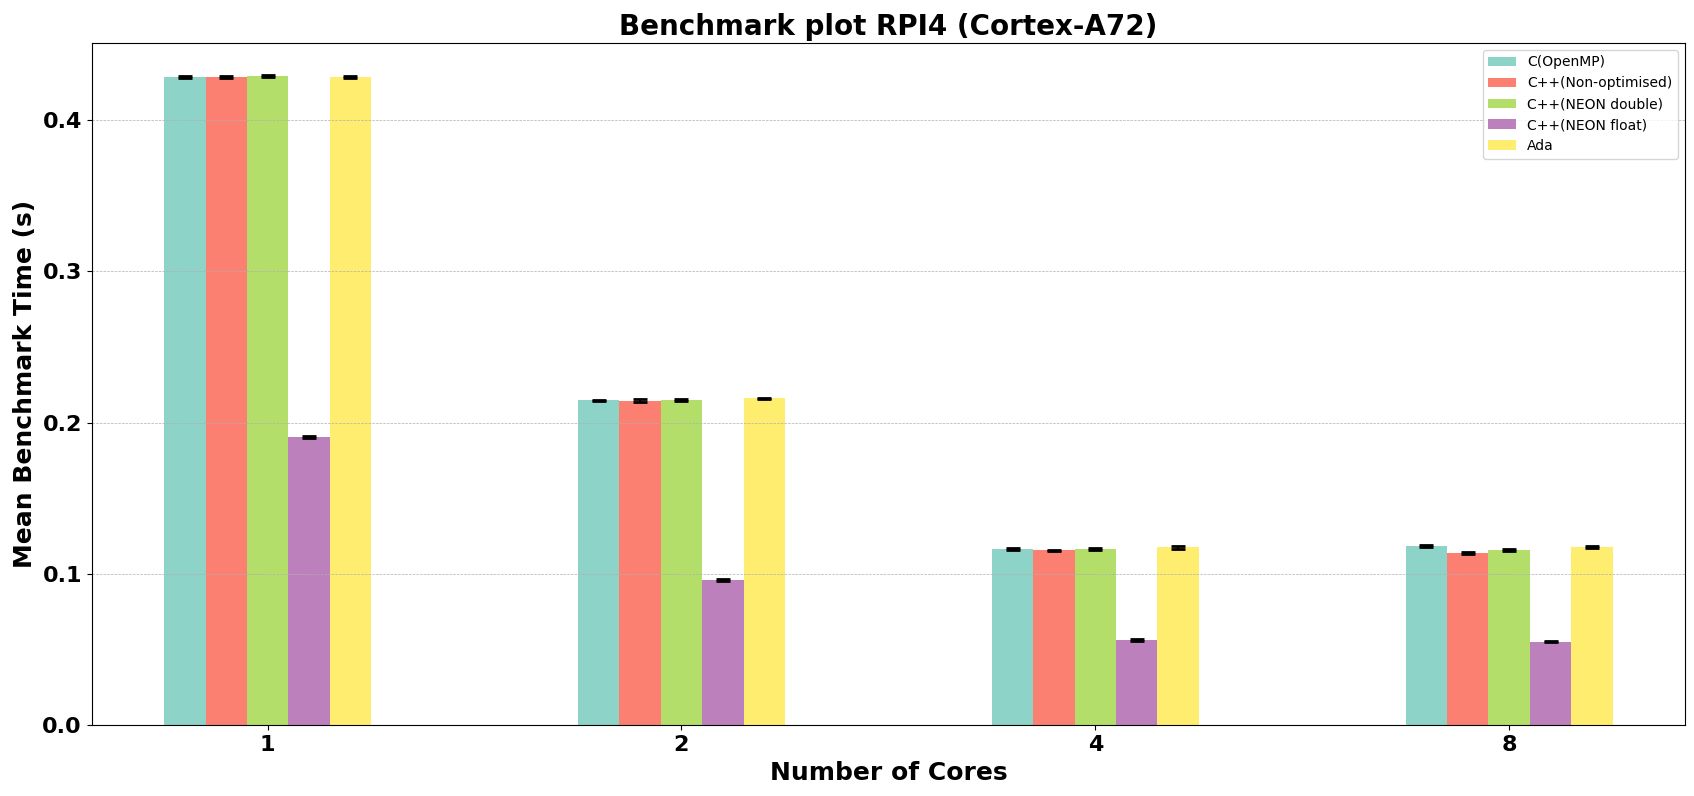
\includegraphics[width=1\textwidth, height=20cm]{~/Documents/Part_D_Modules/Individual_Project/Individual_report/figures/mpbenchmark_rpi4.png} % Adjust the path and width as needed
	\caption{Mean benchmark plot of results collected from Raspberry Pi 4(in seconds). The error bars represent 95\% confidence interval. (Lower is better).}
	\label{fig:mpbenchmark_rpi4_plot} % Use this label to reference the figure
\end{figure}

\begin{figure}[H] % Positioning preference: here, top, bottom, page
	\centering
	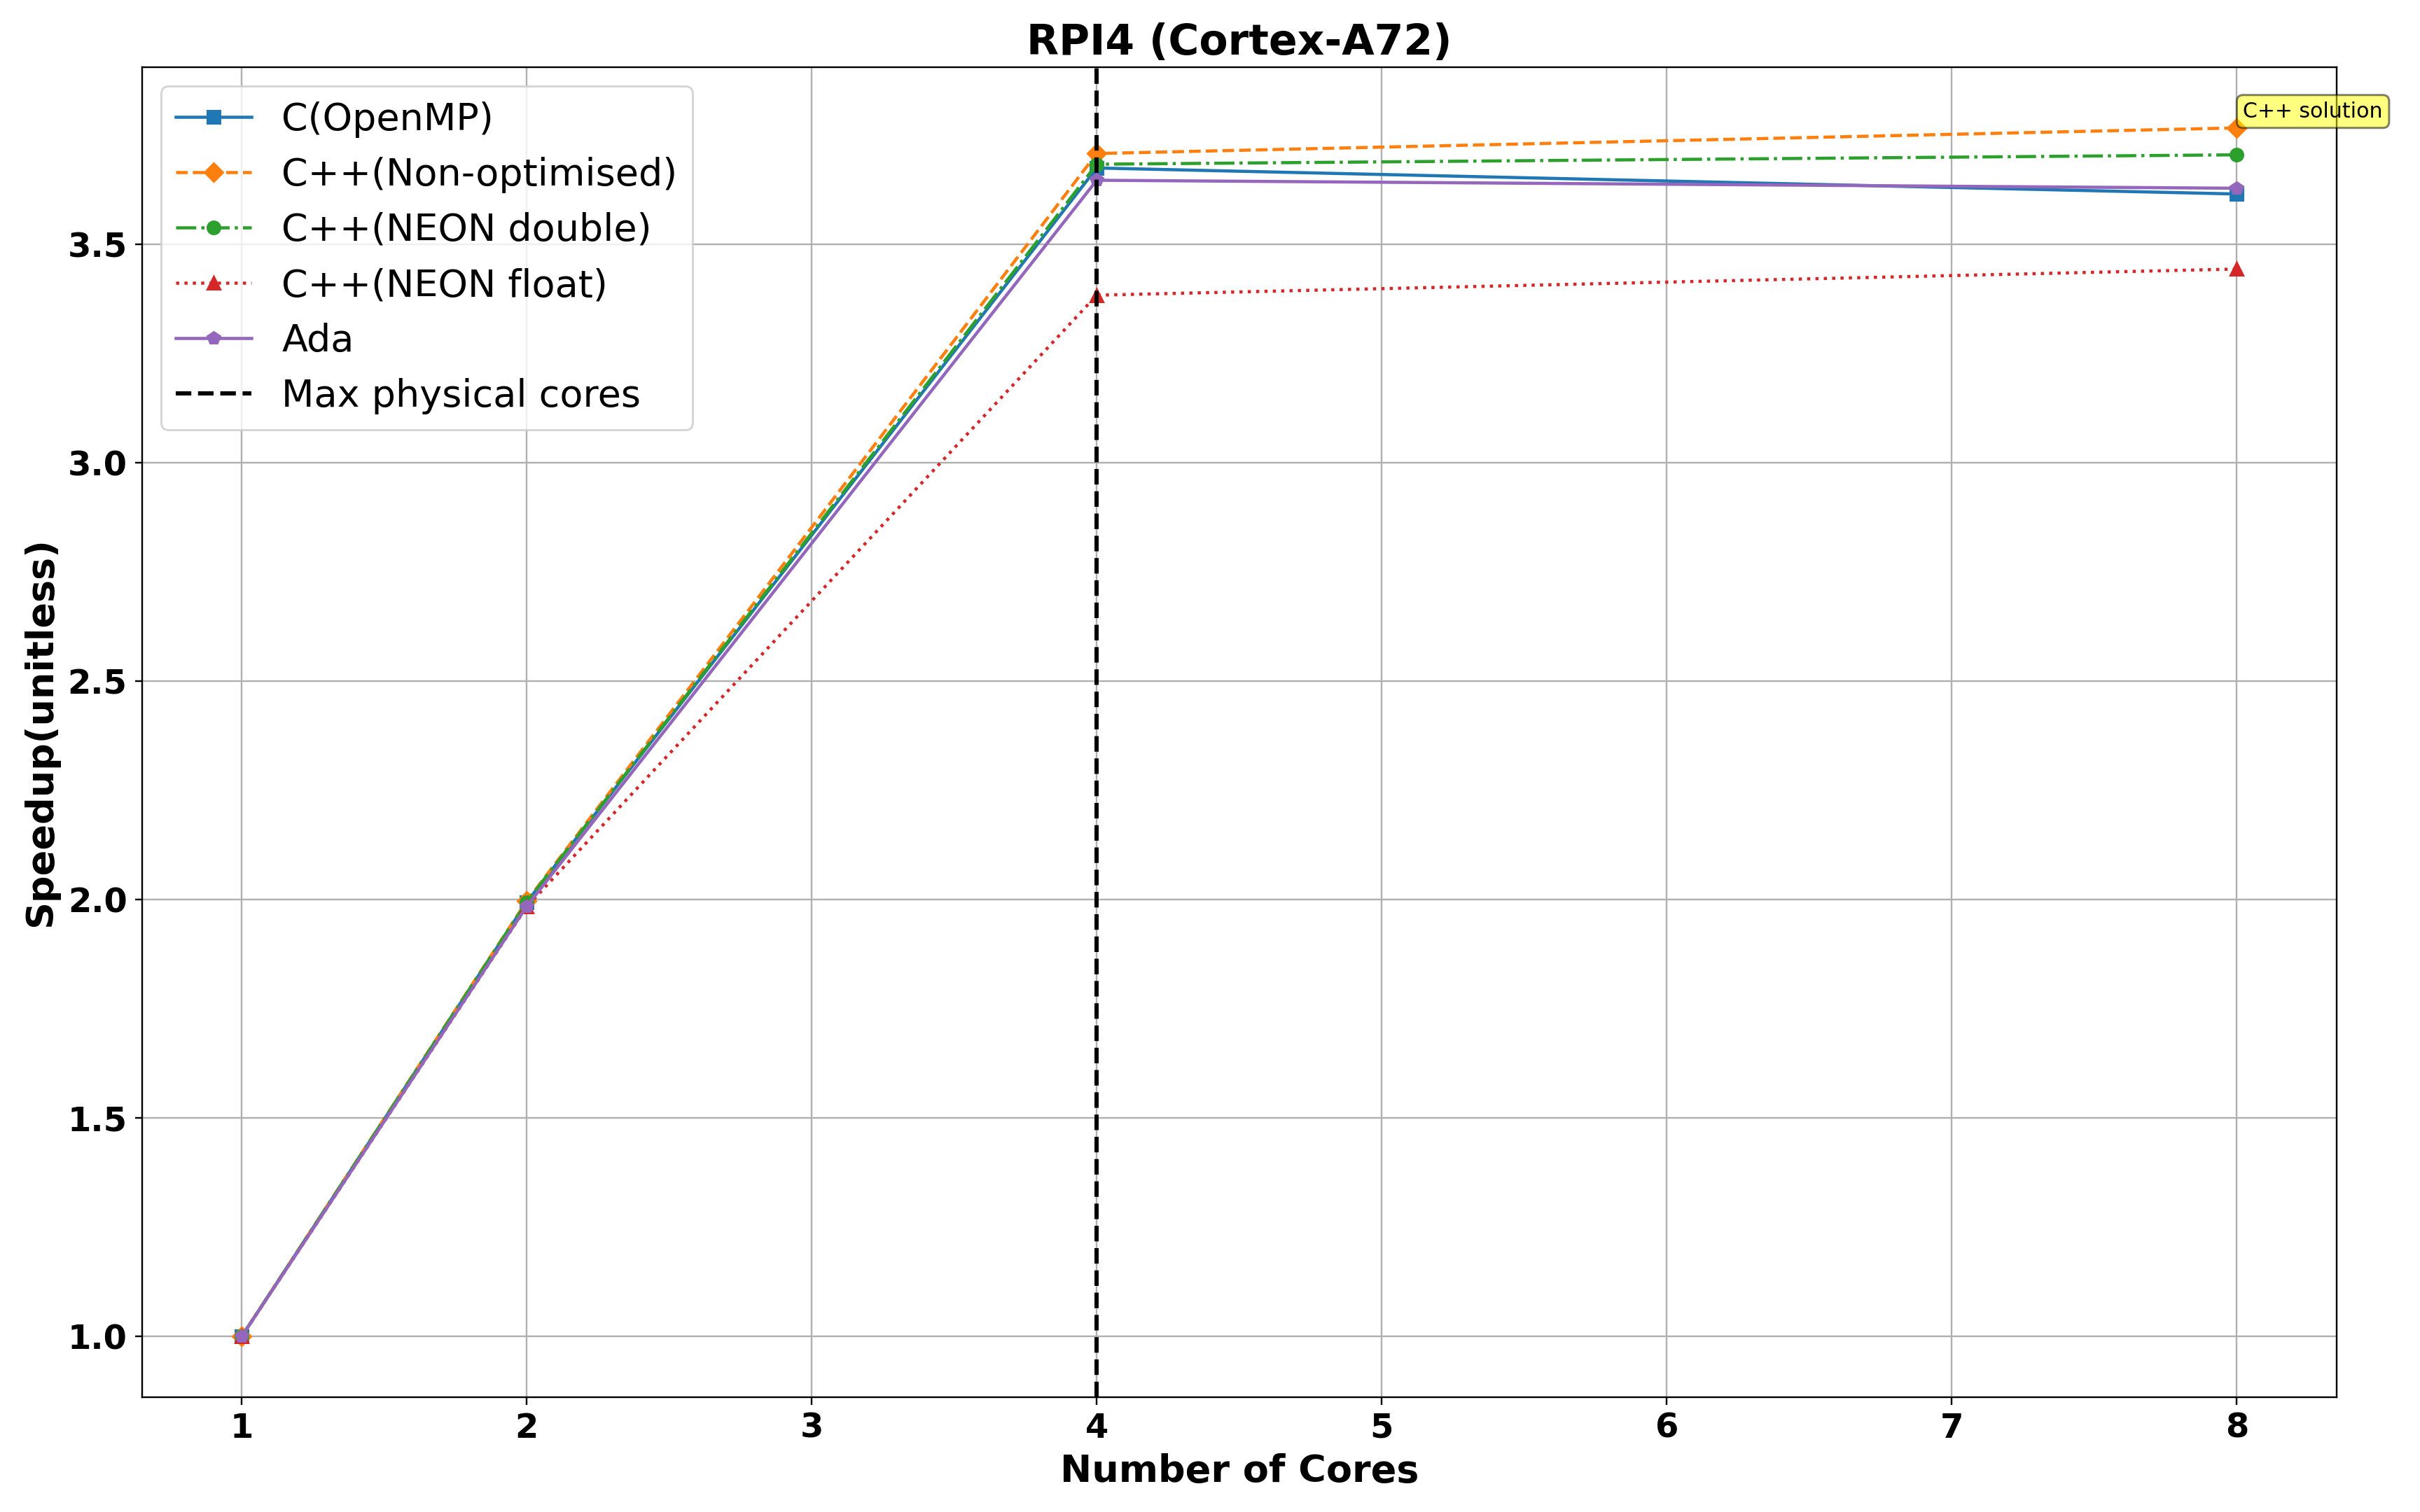
\includegraphics[width=1\textwidth, height=20cm]{~/Documents/Part_D_Modules/Individual_Project/Individual_report/figures/mpbenchmark_rpi4_speedup.png} % Adjust the path and width as needed
	\caption{Speedup plot collected from Raspberry Pi 4 processor. The vertical black line shows the maximum physical cores of the processor. (Higher is better).}
	\label{fig:mpbenchmark_rpi4_speedup_plot} % Use this label to reference the figure
\end{figure}

\section{Objective 2: \texttt{MobileNet}}

\begin{figure}[H] % Positioning preference: here, top, bottom, page
	\centering
	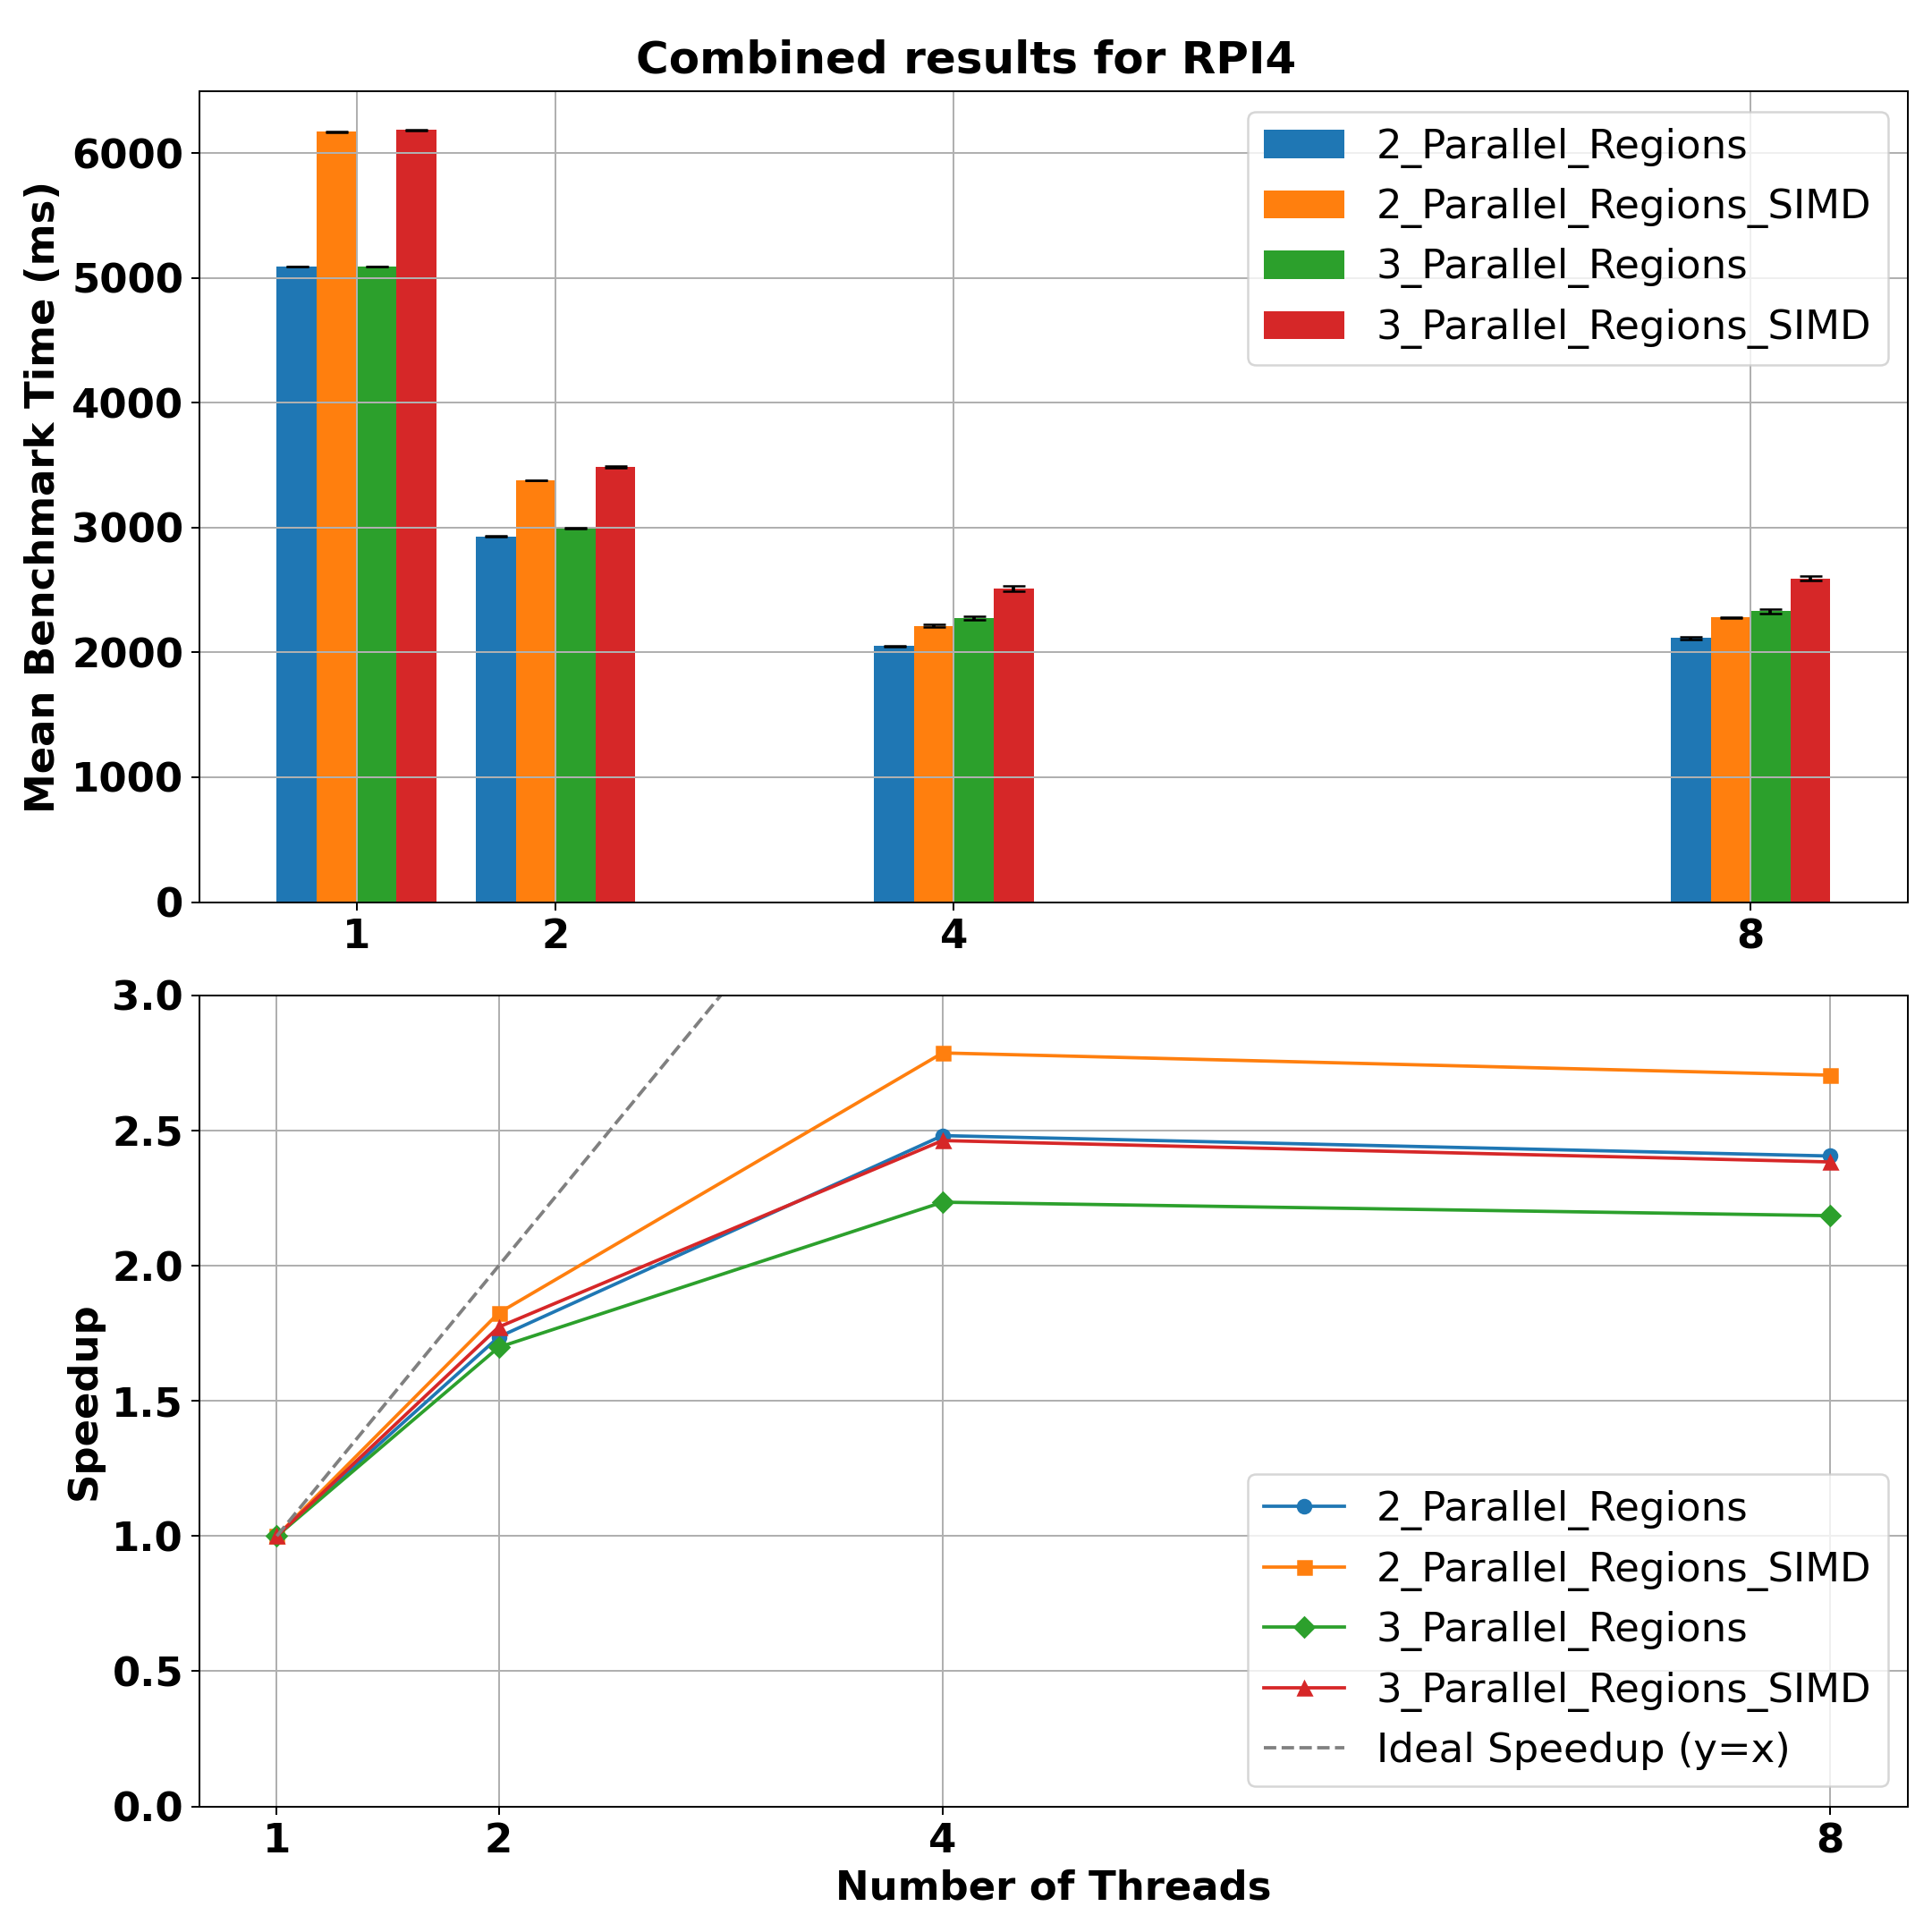
\includegraphics[width=1\textwidth, height=20cm]{~/Documents/Part_D_Modules/Individual_Project/Individual_report/figures/mobilenet_rpi4.png} % Adjust the path and width as needed
	\caption{Mean benchmark plot of results collected from \texttt{Cortex A-72} processor(in milliseconds). (Lower is better).}
	\label{fig:mobilenet_rpi4_plot} % Use this label to reference the figure
\end{figure}

\begin{figure}[H] % Positioning preference: here, top, bottom, page
	\centering
	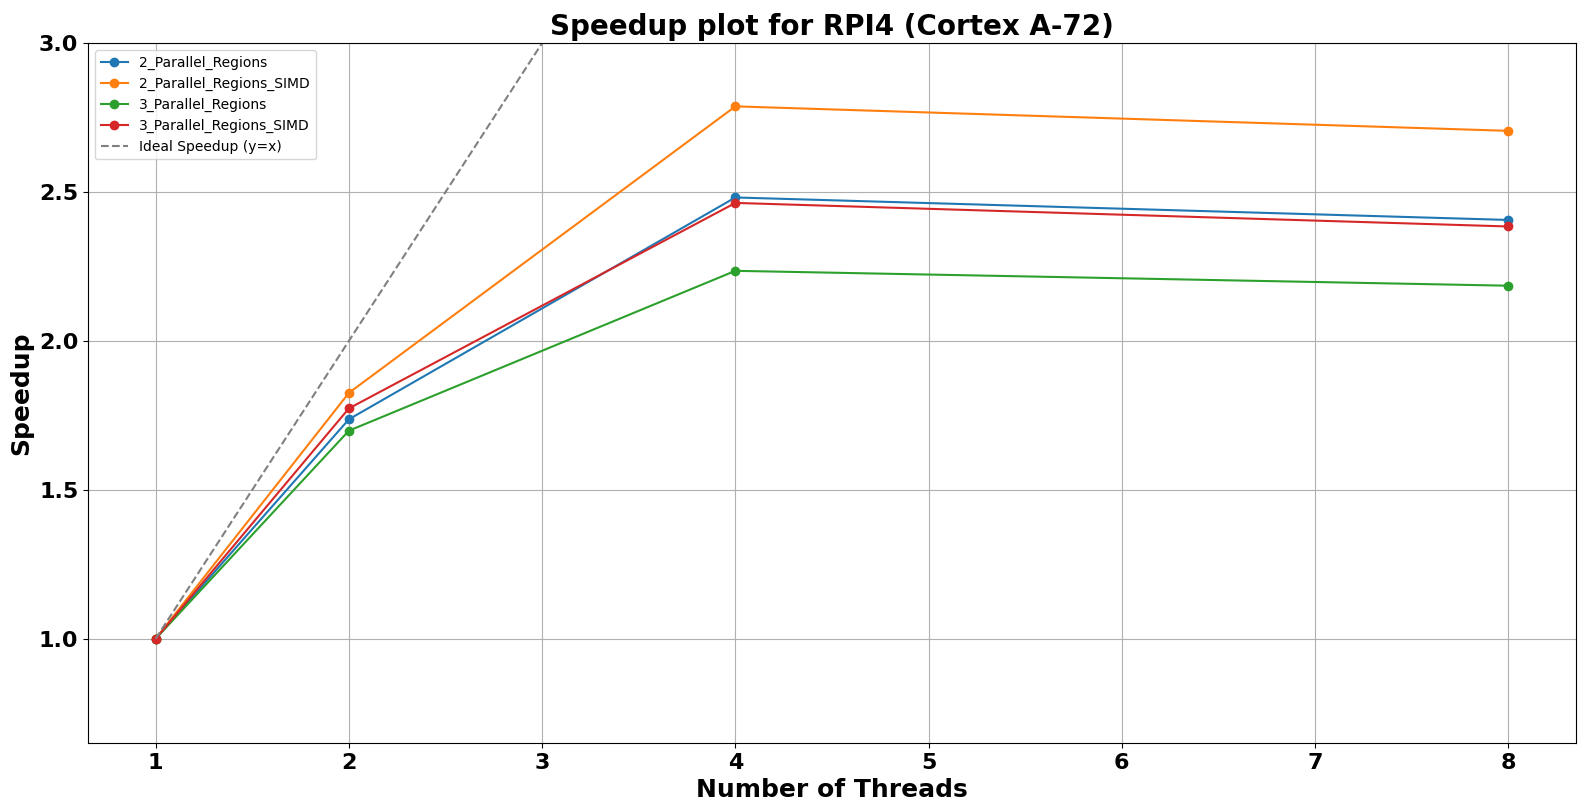
\includegraphics[width=1\textwidth, height=20cm]{~/Documents/Part_D_Modules/Individual_Project/Individual_report/figures/mobilenet_rpi4_speedup.png} % Adjust the path and width as needed
	\caption{Speedup plot comparing different solutions with results collected from \texttt{Cortex A-72} processor. (Higher is better).}
	\label{fig:mobilenet_rpi4_speedup} % Use this label to reference the figure
\end{figure}

\section{Objective 3: \texttt{DeBaTE-FI} platform}

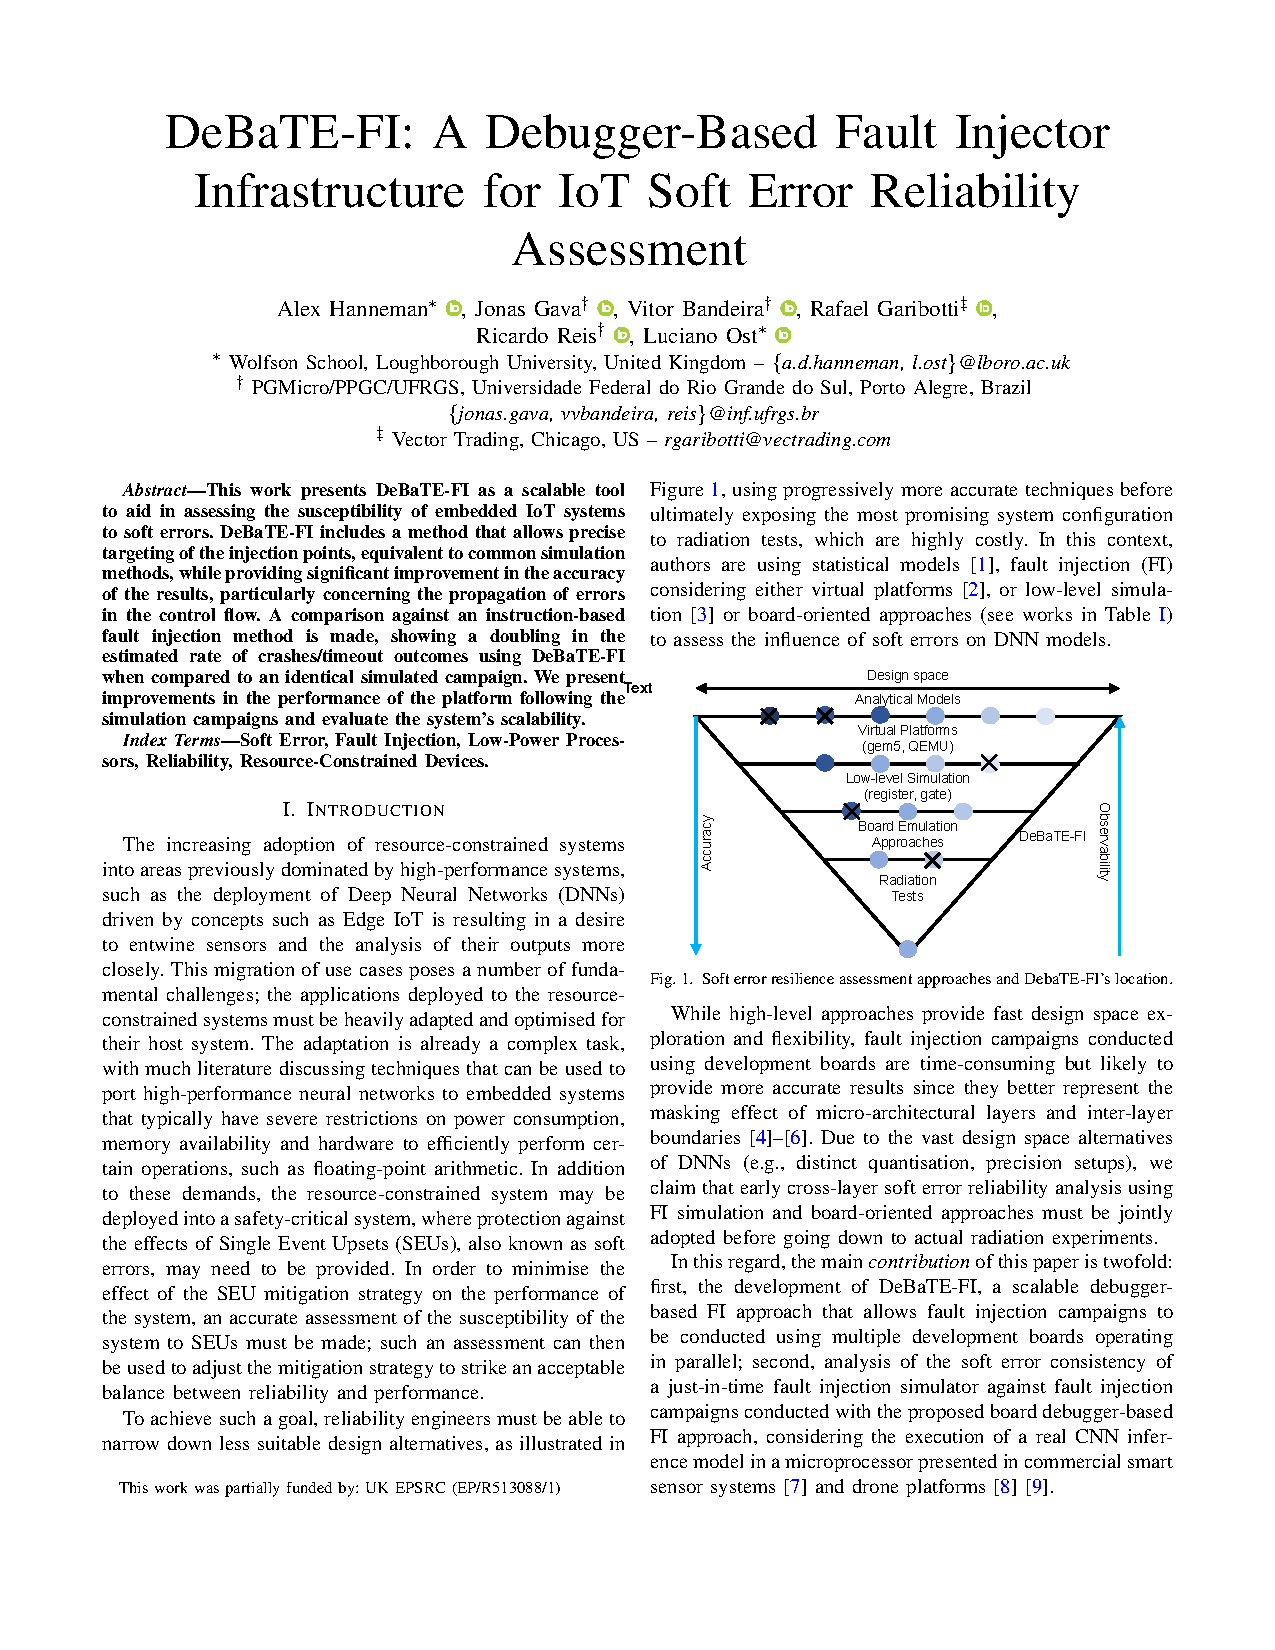
\includepdf[
pages=-,
addtotoc={1, section, 1, DeBaTE-FI platform publication(maybe remove?), appendix:debate_fi},
pagecommand={\label{appendix:debate_fi}}
]{~/Documents/Part_D_Modules/Individual_Project/Individual_report/files/Debate_FI_platform.pdf}


